\documentclass[10pt]{beamer}

% Packages
\usepackage[utf8]{inputenc}
\usepackage[T1]{fontenc}
\usepackage{amsmath, amssymb, amsthm}
\usepackage{graphicx}
\usepackage{booktabs}
\usepackage{hyperref}
\usepackage{tikz}
\usetikzlibrary{shapes,arrows,positioning,calc}

% Theme settings
\usetheme{default}
\usecolortheme{default}
\usefonttheme{professionalfonts}

\definecolor{ImperialBlue}{RGB}{0, 62, 116}
\definecolor{DarkGray}{RGB}{51, 51, 51}
\definecolor{LightGray}{RGB}{245, 245, 245}
\definecolor{AccentOrange}{RGB}{214, 96, 77}
\definecolor{AccentGreen}{RGB}{46, 139, 87}

% Apply colors
\setbeamercolor{frametitle}{fg=ImperialBlue, bg=white}
\setbeamercolor{title}{fg=ImperialBlue}
\setbeamercolor{structure}{fg=ImperialBlue}
\setbeamercolor{normal text}{fg=DarkGray}
\setbeamercolor{block title}{fg=white, bg=ImperialBlue}
\setbeamercolor{block body}{fg=DarkGray, bg=LightGray}
\setbeamercolor{itemize item}{fg=ImperialBlue}
\setbeamercolor{enumerate item}{fg=ImperialBlue}

% Remove navigation symbols
\setbeamertemplate{navigation symbols}{}

% Customize frame title
\setbeamertemplate{frametitle}{
  \vspace{0.5em}
  \insertframetitle
  \vspace{0.3em}
}

% Customize itemize
\setbeamertemplate{itemize items}[circle]
\setlength{\leftmargini}{1.5em}

% Footer
\setbeamertemplate{footline}{
  \leavevmode%
  \hbox{%
  \begin{beamercolorbox}[wd=.333333\paperwidth,ht=2.25ex,dp=1ex,left]{author in head/foot}%
    \hspace{1em}\usebeamerfont{author in head/foot}\insertshortauthor
  \end{beamercolorbox}%
  \begin{beamercolorbox}[wd=.333333\paperwidth,ht=2.25ex,dp=1ex,center]{title in head/foot}%
    \usebeamerfont{title in head/foot}\insertshorttitle
  \end{beamercolorbox}%
  \begin{beamercolorbox}[wd=.333333\paperwidth,ht=2.25ex,dp=1ex,right]{date in head/foot}%
    \usebeamerfont{date in head/foot}\insertshortdate{}\hspace*{2em}
    \insertframenumber{} / \inserttotalframenumber\hspace*{2ex} 
  \end{beamercolorbox}}%
  \vskip0pt%
}

% Commands for highlighting
\newcommand{\emphbox}[1]{\colorbox{LightGray}{\textcolor{DarkGray}{#1}}}
\newcommand{\highlight}[1]{\textcolor{AccentOrange}{\textbf{#1}}}
\newcommand{\good}[1]{\textcolor{AccentGreen}{#1}}
\newcommand{\bad}[1]{\textcolor{AccentOrange}{#1}}

%----------------------------------------------------------------------------------------
\title{Cryptocurrencies as an Asset Class (Part II)}
\subtitle{ECOM215: Blockchain Economics and Digital Assets}
\author{Dr Daniele Bianchi}
\institute{Queen Mary, University of London}
\date{Semester B, 2025/2026}
%----------------------------------------------------------------------------------------

\begin{document}

\AtBeginSection[]{
  \begin{frame}[plain]
    \vfill
    \begin{center}
      {\Large\color{ImperialBlue}\insertsection}
    \end{center}
    \vfill
  \end{frame}
}

\begin{frame}[plain]
  \titlepage
\end{frame}

\begin{frame}{Today's Agenda}
  \tableofcontents
\end{frame}

%----------------------------------------------------------------------------------------
\section{Recap and Motivation}
%----------------------------------------------------------------------------------------

\begin{frame}{Where We Left Off}
  \textbf{Last lecture} we established the foundations:
  \begin{itemize}
    \item Crypto markets are structurally different from traditional markets (fragmented, 24/7, custody risk)
    \item Valuation is fundamentally challenging---no cash flows, alternative frameworks are suggestive but unreliable
    \item Returns have been high but volatility and drawdowns are extreme
    \item The diversification benefit has weakened as correlations with equities increased
  \end{itemize}
  
  \vspace{1em}
  \textbf{This lecture} we ask: Given all of that, \highlight{how do investors actually access crypto markets?}
  
  \vspace{0.5em}
  \begin{itemize}
    \item The regulatory breakthrough that enabled institutional access (ETFs)
    \item The full menu of investment vehicles (direct and indirect)
    \item The risks that regulation has not yet solved (manipulation, fraud)
  \end{itemize}
\end{frame}

%----------------------------------------------------------------------------------------
\section{The 2024 Spot ETF Approvals}
%----------------------------------------------------------------------------------------

\begin{frame}{Why ETFs Matter}
  \textbf{Exchange-Traded Funds (ETFs)} are investment vehicles that:
  \begin{itemize}
    \item Trade on regulated stock exchanges (like ordinary shares)
    \item Track the price of an underlying asset or basket of assets
    \item Provide exposure \textit{without} requiring investors to hold the asset directly
  \end{itemize}
  
  \vspace{0.5em}
  \textbf{Why this is transformative for crypto:}
  \begin{enumerate}
    \item \textbf{Accessibility}: Any investor with a brokerage account can buy---no wallets, no private keys, no exchanges
    \item \textbf{Regulatory wrapper}: ETFs are regulated securities products with investor protections
    \item \textbf{Institutional mandates}: Many pension funds, endowments, and wealth managers \textit{cannot} hold crypto directly but \textit{can} hold ETFs
    \item \textbf{Tax and reporting}: Standard tax treatment, integrated into existing portfolio reporting
  \end{enumerate}
  
  \vspace{0.5em}
  The approval of \highlight{spot} crypto ETFs in 2024 was the single most significant event for crypto's integration into traditional finance.
\end{frame}

\begin{frame}{Spot vs.\ Futures ETFs: A Critical Distinction}
  \textbf{Futures-based ETFs} (e.g., ProShares BITO, approved October 2021):
  \begin{itemize}
    \item Hold CME Bitcoin futures contracts, not actual Bitcoin
    \item Must ``roll'' contracts---selling expiring futures, buying new ones
    \item \textbf{Roll cost}: when futures trade at a premium to spot (\textit{contango}), rolling destroys value over time.
%    \item Tracking error relative to Bitcoin's spot price can be substantial
  \end{itemize}
  
  \vspace{0.5em}
  \textbf{Spot ETFs} (approved January 2024):
  \begin{itemize}
    \item Hold actual Bitcoin in custody through a qualified custodian
    \item Price tracks the spot market directly
    \item No roll cost, no contango drag
  \end{itemize}
  
  \vspace{0.5em}
  \begin{block}{Why the Distinction Matters}
    The SEC approved futures ETFs in 2021 but resisted spot ETFs for years, arguing that the spot market was susceptible to manipulation. This reflects a fundamental regulatory judgment about market integrity.
  \end{block}
\end{frame}

\begin{frame}{The Road to Approval: A Decade of Rejection}
  The SEC rejected spot BTC ETF applications from 2013 to 2023.
  
  \vspace{0.5em}
  \textbf{Timeline of key events:}
  \begin{center}
    \small
    \begin{tabular}{ll}
      \toprule
      \textbf{Date} & \textbf{Event} \\
      \midrule
      2013 & Winklevoss twins file first Bitcoin ETF application \\
      2017 & SEC rejects Winklevoss ETF; cites market manipulation risk \\
      2021 & Futures-based ETFs approved (ProShares BITO) \\
      2021 & Grayscale files to convert GBTC trust to spot ETF; SEC rejects \\
      2023 (Jun) & BlackRock files for iShares Bitcoin Trust (IBIT) \\
      2023 (Aug) & Court rules in \textit{Grayscale v.\ SEC}: rejection was \\
       & ``arbitrary and capricious'' \\
      2024 (Jan) & SEC approves 11 spot Bitcoin ETFs simultaneously \\
      2024 (May) & SEC approves spot Ethereum ETFs \\
      \bottomrule
    \end{tabular}
  \end{center}
  
  \vspace{0.3em}
  The \textit{Grayscale v.\ SEC} ruling was decisive: the court found the SEC could not logically approve futures ETFs while rejecting spot ETFs, since both reference the same underlying market.
\end{frame}

\begin{frame}{The SEC's Concerns and How They Were Addressed}
  \textbf{The SEC's core objection} was market manipulation in the unregulated spot market.
  
  \vspace{0.5em}
  \textbf{Specific concerns:}
  \begin{itemize}
    \item No regulated market of ``significant size'' for price discovery
    \item Wash trading and potential for fraud with no market surveillance
  \end{itemize}
  
  \vspace{0.5em}
  \textbf{What changed:}
  \begin{itemize}
    \item \textbf{CME futures market matured}: Deep liquidity, regulated, with surveillance---the SEC accepted that CME futures \textit{lead} price discovery
    \item \textbf{Qualified custody}: Coinbase Custody (regulated by NYDFS) designated as custodian for most approved ETFs
    \item \textbf{The court forced the issue}: After losing \textit{Grayscale}, the SEC's legal position was untenable
  \end{itemize}
  
  \vspace{0.3em}
  \begin{block}{Note}
    SEC Chair Gensler emphasised that approval of Bitcoin ETFs did \textit{not} constitute SEC endorsement of Bitcoin itself. The SEC approved a \textit{product structure}, not the underlying asset.
  \end{block}
\end{frame}

\begin{frame}{How Spot Bitcoin ETFs Work}
  % TikZ diagram showing the creation/redemption mechanism
  \begin{center}
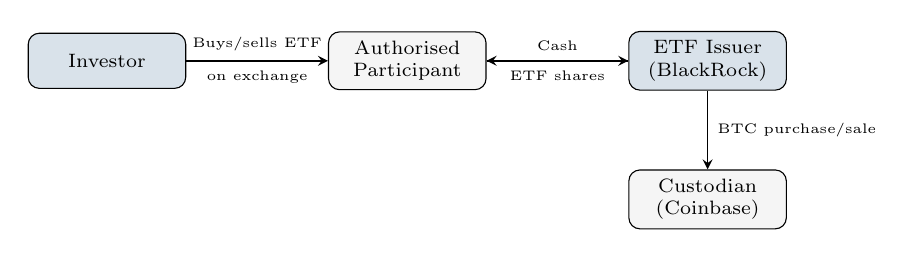
\begin{tikzpicture}[
    node distance=1cm and 1.8cm,
    box/.style={draw, rectangle, rounded corners, minimum width=2cm, minimum height=0.7cm, align=center, font=\scriptsize, fill=LightGray},
    bluebox/.style={draw, rectangle, rounded corners, minimum width=2cm, minimum height=0.7cm, align=center, font=\scriptsize, fill=ImperialBlue!15},
    arrow/.style={->, semithick, >=stealth}
  ]
    \node[bluebox] (investor) {Investor};
    \node[box, right=of investor] (ap) {Authorised\\Participant};
    \node[bluebox, right=of ap] (etf) {ETF Issuer\\(BlackRock)};
    \node[box, below=1cm of etf] (custodian) {Custodian\\(Coinbase)};
    
    \draw[arrow] (investor) -- node[above, font=\tiny] {Buys/sells ETF} node[below, font=\tiny] {on exchange} (ap);
    \draw[arrow] (ap) -- node[above, font=\tiny] {Cash} (etf);
    \draw[arrow] (etf) -- node[below, font=\tiny] {ETF shares} (ap);
    \draw[arrow] (etf) -- node[right, font=\tiny] {BTC purchase/sale} (custodian);
  \end{tikzpicture}
  \end{center}
  
  \vspace{0.3em}
  \textbf{Key design feature---cash creation/redemption:}
  \begin{itemize}
    \item The SEC required \textbf{cash-only} creation/redemption (no in-kind BTC delivery)
    \item APs deliver cash to the issuer, who then buys Bitcoin on the market
    \item This adds a small layer of friction and cost compared to in-kind ETFs (e.g., equity or gold ETFs), but avoids broker-dealers handling Bitcoin directly
  \end{itemize}
\end{frame}

\begin{frame}{ETF Flows and the Fee War}
  The launch of spot Bitcoin ETFs was one of the most successful ETF debuts in history.
  
  \vspace{0.5em}
  \textbf{Key data points (as of early 2025):}
  \begin{itemize}
    \item Combined net inflows exceeded \$30 billion in the first year
    \item iShares Bitcoin Trust (IBIT) alone surpassed \$50 billion in AUM, making it one of the fastest-growing ETFs ever launched
    \item Grayscale's GBTC experienced significant \textit{outflows} as investors rotated from the legacy trust (1.5\% fee) into cheaper alternatives
  \end{itemize}
  
  % \vspace{0.3em}
  % % FIGURE PLACEHOLDER: Cumulative net flows into spot Bitcoin ETFs (stacked by issuer)
  % % Source: The Block — "Bitcoin ETF Flows" or Farside Investors
  % % Suggestion: Show IBIT, FBTC, GBTC separately to illustrate the rotation story
  % \textit{[Figure: Cumulative net flows into spot Bitcoin ETFs by issuer. Source: theblock.co / Farside Investors]}
  
  \vspace{0.3em}
  \textbf{The fee war:}
  \begin{center}
    \small
    \begin{tabular}{lcc}
      \toprule
      \textbf{ETF} & \textbf{Issuer} & \textbf{Expense ratio} \\
      \midrule
      IBIT & BlackRock & 0.25\% \\
      FBTC & Fidelity & 0.25\% \\
      ARKB & ARK/21Shares & 0.21\% \\
      GBTC & Grayscale & 1.50\% \\
      BTC (mini) & Grayscale & 0.15\% \\
      \bottomrule
    \end{tabular}
  \end{center}
\end{frame}

\begin{frame}{ETF Flows and the Fee War}

\begin{figure}
    \centering
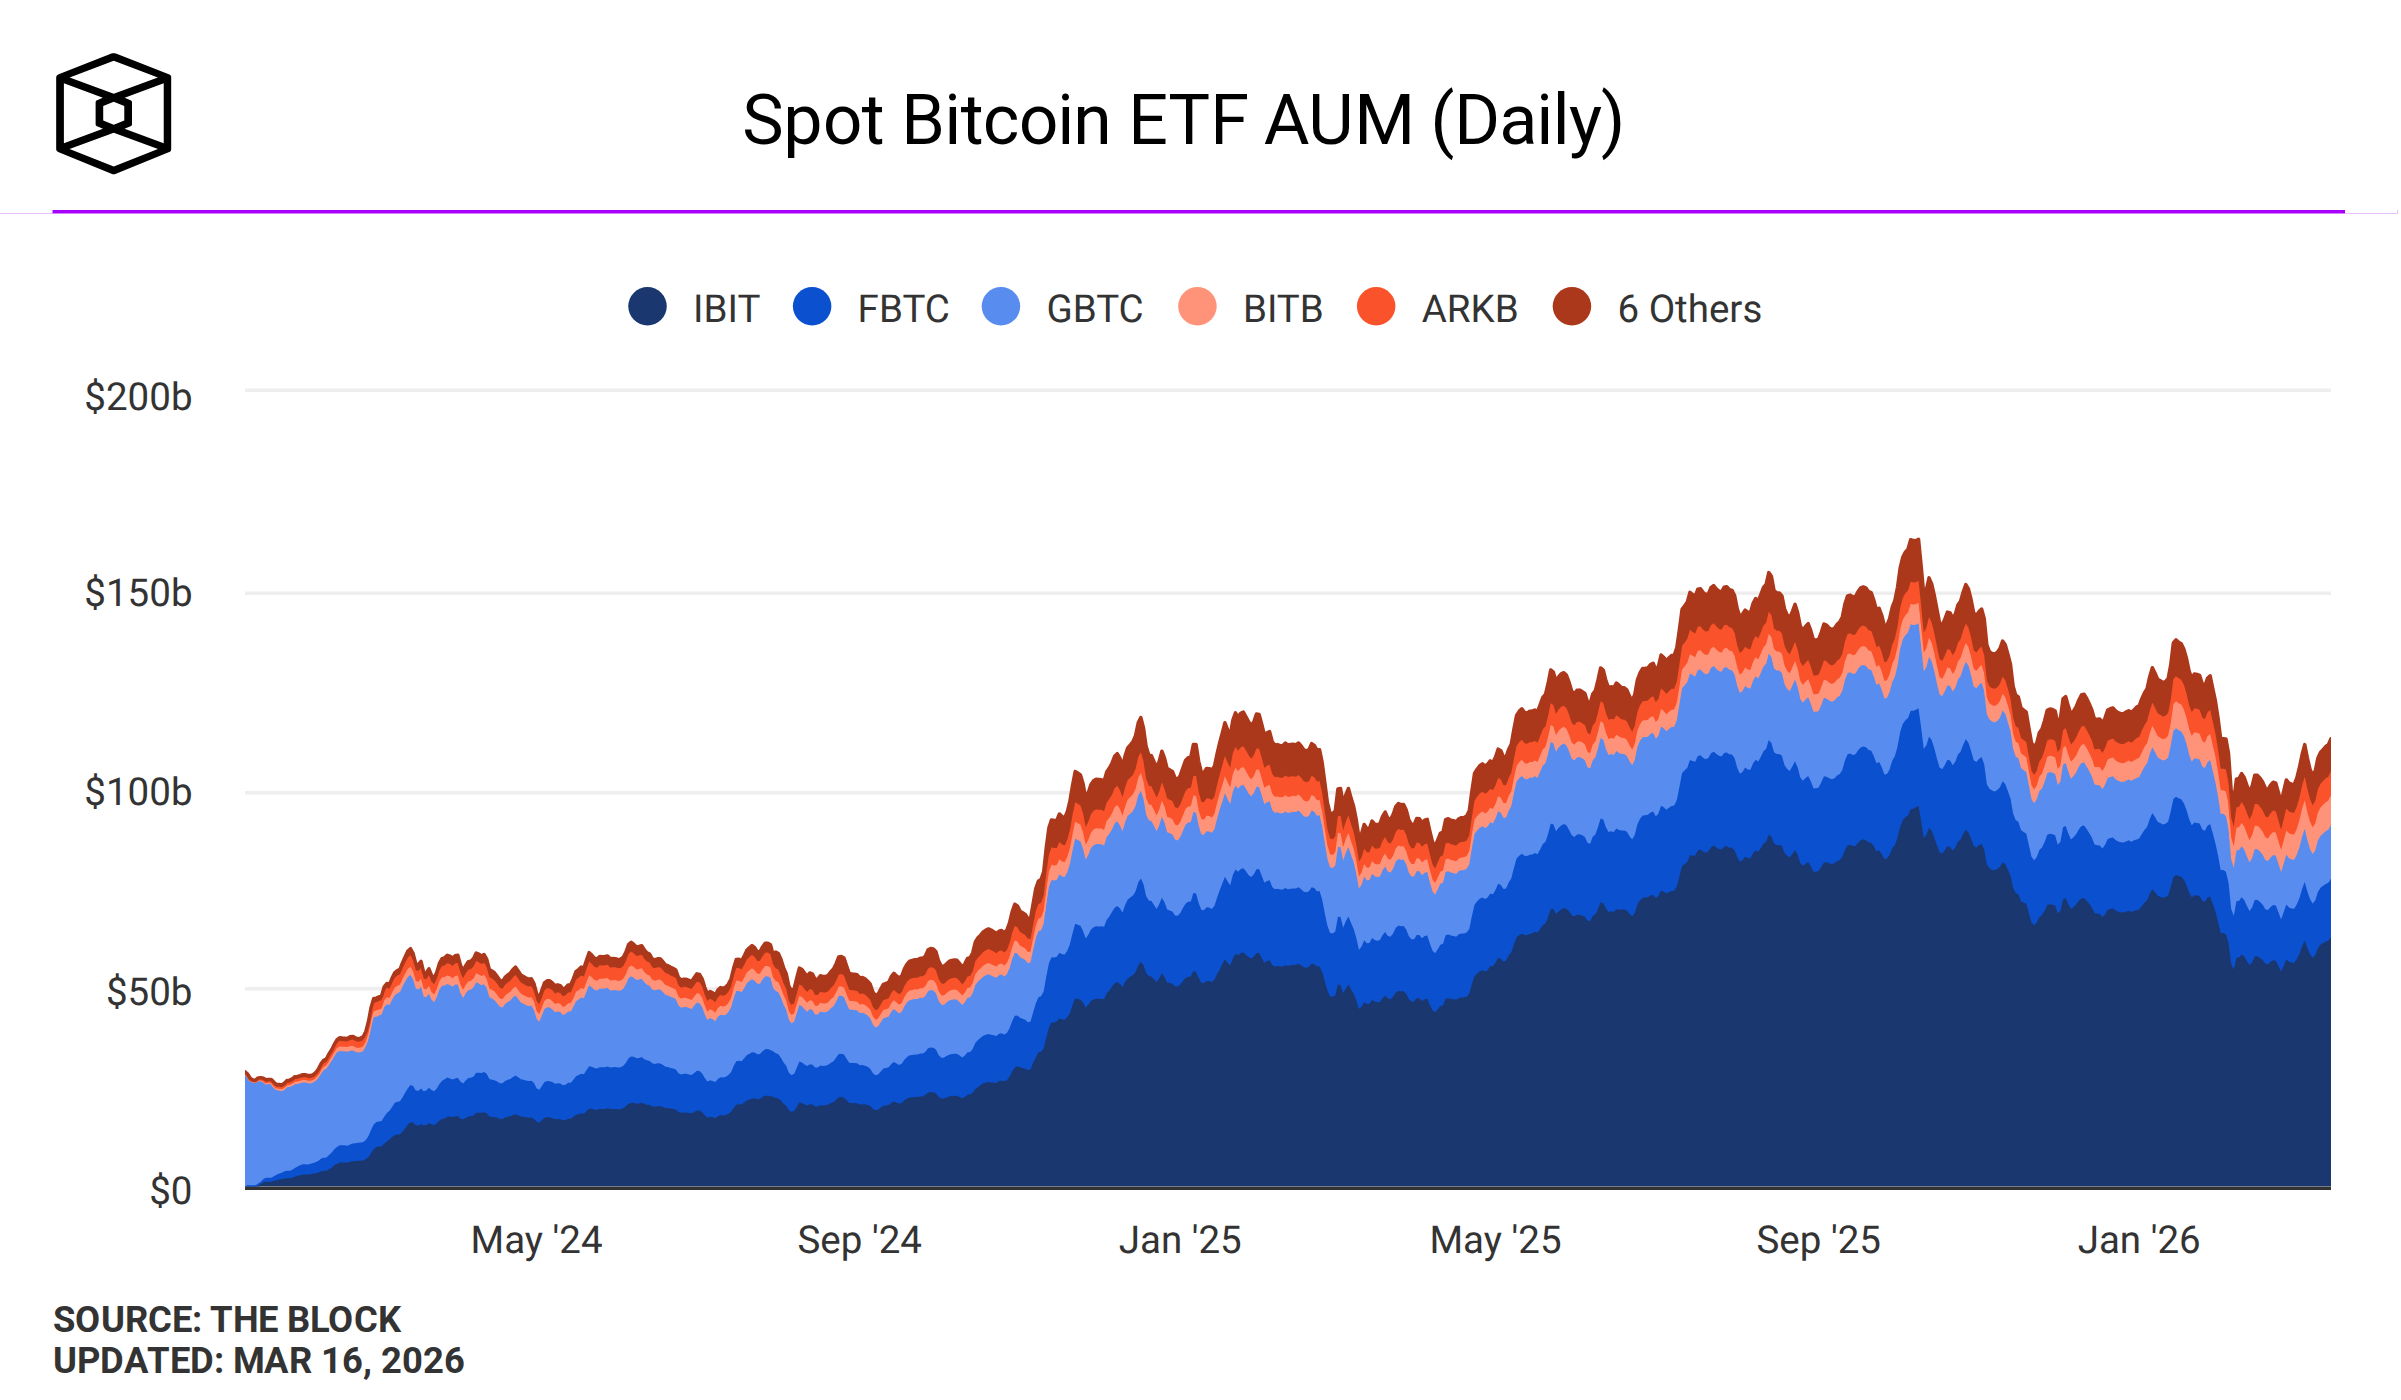
\includegraphics[width=1\linewidth]{Figures/spot-bitcoin-etf-onchain-holdings-usd.png}
\caption{Cumulative Asset Under Management (AUM) into spot Bitcoin ETFs by issuer. Source: theblock.co}
    \label{fig:BTC ETF}
\end{figure}  
  
\end{frame}


\begin{frame}{Ethereum Spot ETFs}
  In May 2024, the SEC also approved spot Ethereum ETFs.
  
  \vspace{0.5em}
  \textbf{Key differences from Bitcoin ETFs:}
  \begin{itemize}
    \item \textbf{No staking}: The SEC required that ETH held by ETFs \textit{not} be staked. This means ETF holders forgo the $\sim$3--4\% staking yield---a significant economic cost.
    \item \textbf{Lower demand}: ETH ETF inflows were substantially smaller than BTC ETFs, reflecting lower institutional demand and the staking restriction.
    \item \textbf{Narrative complexity}: Bitcoin's ``digital gold'' pitch is simple; Ethereum's value proposition (programmable platform, fee revenue, DeFi ecosystem) is harder to convey to traditional allocators.
  \end{itemize}
  
  % \vspace{0.5em}
  % % FIGURE PLACEHOLDER: Comparison of BTC vs ETH ETF cumulative flows since launch
  % % Source: The Block or Farside Investors
  % \textit{[Figure: Cumulative flows---Bitcoin spot ETFs vs.\ Ethereum spot ETFs. Source: theblock.co]}
  
  \vspace{0.3em}
  \begin{block}{Open Question}
    If the SEC eventually permits staking within ETH ETFs, the product becomes considerably more attractive---investors would earn yield on top of price exposure. This decision remains pending.
  \end{block}
\end{frame}

\begin{frame}{Ethereum Spot ETFs}

\begin{figure}
    \centering
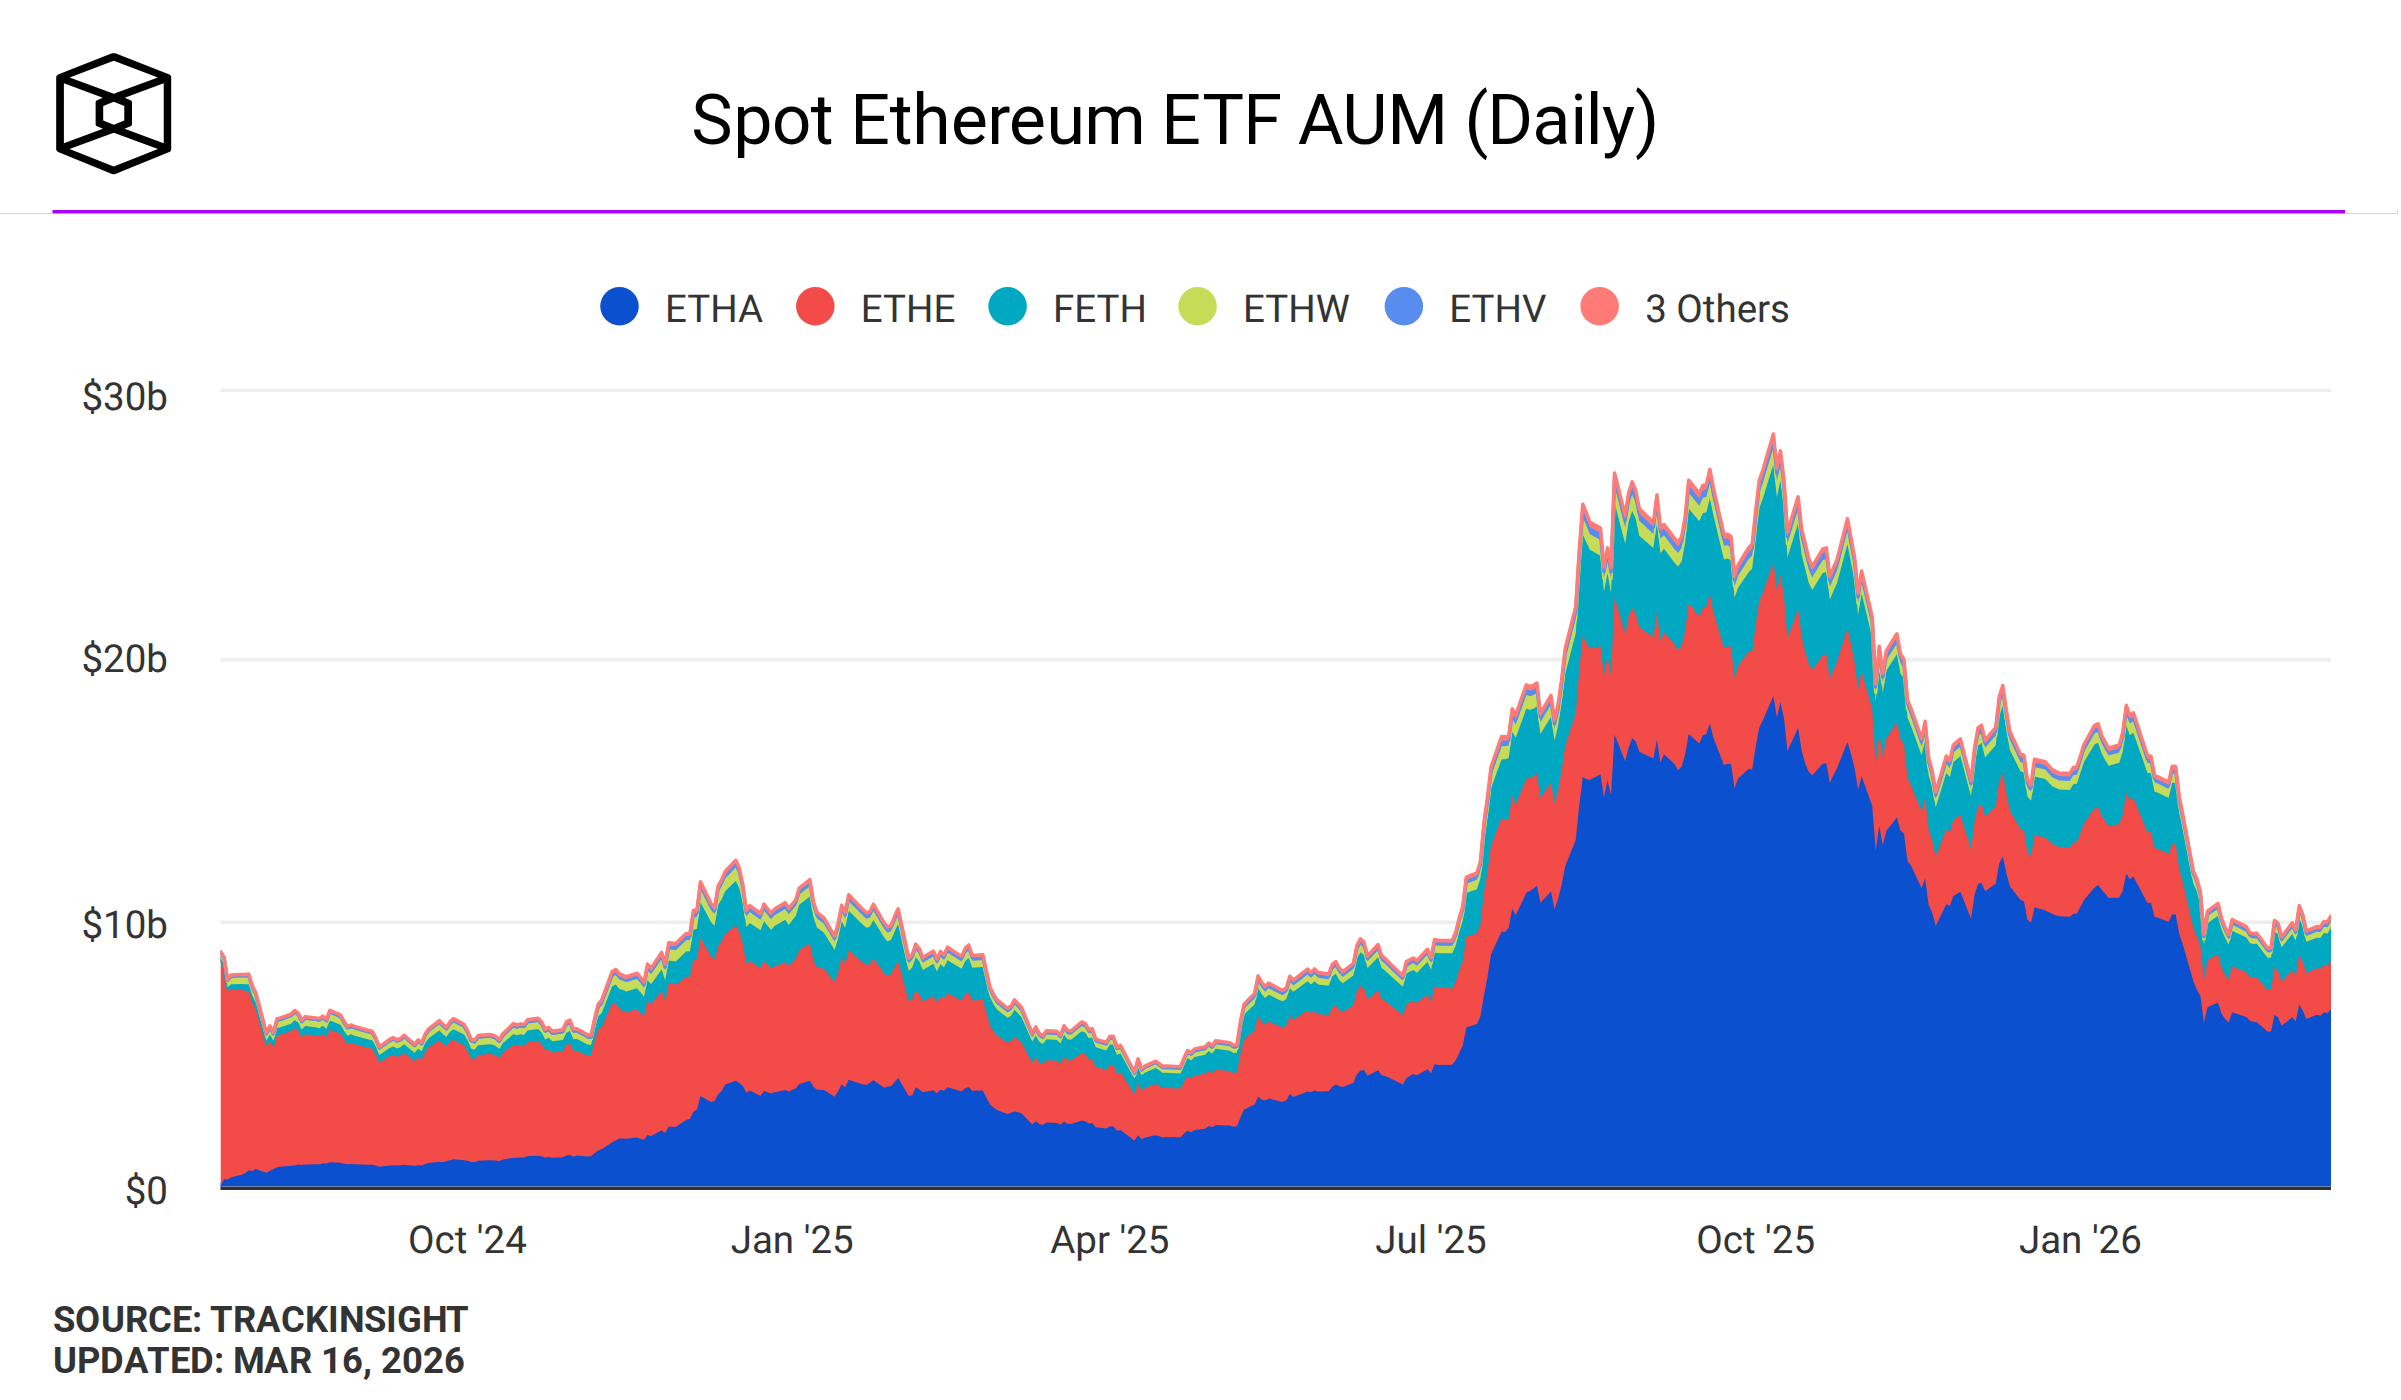
\includegraphics[width=1\linewidth]{Figures/spot-ethereum-etf-aum-daily.png}
\caption{Cumulative Asset Under Management (AUM) into spot Ethereum ETFs by issuer. Source: theblock.co}
    \label{fig:BTC ETF}
\end{figure} 

  % \vspace{0.5em}
  % % FIGURE PLACEHOLDER: Comparison of BTC vs ETH ETF cumulative flows since launch
  % % Source: The Block or Farside Investors
  % \textit{[Figure: Cumulative flows---Bitcoin spot ETFs vs.\ Ethereum spot ETFs. Source: theblock.co]}

\end{frame}


\begin{frame}{ETF Impact on Price Discovery and Market Structure}
  The introduction of spot ETFs has changed \textit{how} Bitcoin's price is formed.
  
  \vspace{0.5em}
  \textbf{Observed effects:}
  \begin{itemize}
    \item \textbf{Reduced volatility}: Daily volatility declined in the months following ETF launch, consistent with broader, more stable participation
    \item \textbf{Stronger link to macro}: ETF flows respond to equity market sentiment, CPI data, and Fed signalling---reinforcing the correlation increase discussed last week
    \item \textbf{Volume shift}: A growing share of Bitcoin ``exposure'' now trades on regulated US equity exchanges rather than crypto-native venues
  \end{itemize}
  
  \vspace{0.5em}
  \textbf{Economic interpretation}: ETFs have improved market efficiency and access, but at the cost of making Bitcoin behave more like a traditional risk asset. The diversification benefit weakens as the asset becomes more mainstream.
\end{frame}

%----------------------------------------------------------------------------------------
\section{Institutional Adoption}
%----------------------------------------------------------------------------------------

\begin{frame}{The Institutional Ecosystem}
  ETFs were the catalyst, but institutional adoption requires a broader infrastructure:
  
  \vspace{0.5em}
  \begin{center}
  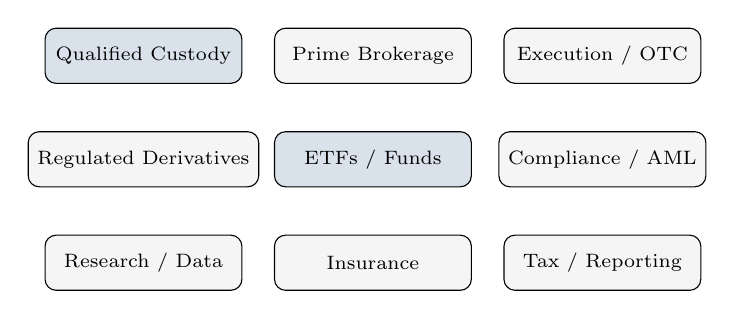
\begin{tikzpicture}[
    node distance=0.6cm and 0.4cm,
    box/.style={draw, rectangle, rounded corners, minimum width=2.5cm, minimum height=0.7cm, align=center, font=\scriptsize, fill=LightGray},
    bluebox/.style={draw, rectangle, rounded corners, minimum width=2.5cm, minimum height=0.7cm, align=center, font=\scriptsize, fill=ImperialBlue!15},
  ]
    \node[bluebox] (custody) {Qualified Custody};
    \node[box, right=of custody] (prime) {Prime Brokerage};
    \node[box, right=of prime] (exec) {Execution / OTC};
    
    \node[box, below=of custody] (deriv) {Regulated Derivatives};
    \node[bluebox, below=of prime] (etfs) {ETFs / Funds};
    \node[box, below=of exec] (compliance) {Compliance / AML};
    
    \node[box, below=of deriv] (research) {Research / Data};
    \node[box, below=of etfs] (insurance) {Insurance};
    \node[box, below=of compliance] (tax) {Tax / Reporting};
  \end{tikzpicture}
  \end{center}
  
  \vspace{0.3em}
  Each layer had to be built before institutions could participate at scale. This infrastructure was largely absent before 2020 and is now substantially in place for BTC and ETH---though still incomplete for smaller assets.
\end{frame}

\begin{frame}{Custody Solutions}
  As discussed last week, institutional custody is a \highlight{prerequisite} for large-scale allocation.
  
  \vspace{0.5em}
  \textbf{Major qualified custodians:}
  \begin{itemize}
    \item \textbf{Coinbase Custody}: Custodian for the majority of US spot ETFs (IBIT, ARKB, and others). Regulated by NYDFS.
    \item \textbf{Fidelity Digital Assets}: Custodian for Fidelity's own FBTC. Operates under existing trust company charter.
    \item \textbf{BitGo}: Independent custodian; insurance-backed; widely used by funds and family offices.
  \end{itemize}
  
  \vspace{0.5em}
  \textbf{The concentration risk:}
  \begin{itemize}
    \item Coinbase custodies a very large share of institutionally held Bitcoin
    \item A single point of failure---operational, regulatory, or security---would have systemic consequences
    \item This is a recognised risk that has not yet been fully mitigated
  \end{itemize}
\end{frame}

\begin{frame}{Corporate Treasuries: The MicroStrategy Model}
  Some publicly listed companies have allocated corporate treasury reserves to Bitcoin.
  
  \vspace{0.5em}
  \textbf{MicroStrategy (now ``Strategy''):}
  \begin{itemize}
    \item Began purchasing Bitcoin in August 2020 under CEO Michael Saylor
    \item Accumulated +400,000 BTC by 2025; the largest corporate holder
    \item Funded purchases through a combination of cash, debt issuance, and equity raises (convertible notes, at-the-market share offerings)
    \item Stock price has become a leveraged proxy for Bitcoin
  \end{itemize}
  
  \vspace{0.5em}
  \textbf{Economic assessment:}
  \begin{itemize}
    \item \good{Shareholders gain BTC exposure through a listed equity with no management fee}
    \item \bad{Leveraged strategy}: If Bitcoin declines significantly, debt servicing becomes difficult and the company faces forced selling pressure
    \item The strategy works spectacularly in bull markets and is extremely dangerous in bear markets
  \end{itemize}
  
  \vspace{0.3em}
  Other adopters (Tesla, Block) have taken much smaller positions. The MicroStrategy model remains an outlier, not a template.
\end{frame}

\begin{frame}{Derivatives Markets}
  Derivatives have become a major component of crypto market structure, often exceeding spot volume.
  
  \vspace{0.5em}
  \textbf{Key instruments:}
  
  \vspace{0.3em}
  \textbf{1.\ Perpetual futures} (crypto-native innovation):
  \begin{itemize}
    \item No expiry date---held indefinitely
    \item \textbf{Funding rate mechanism}: Periodic payments between longs and shorts to keep the contract price aligned with spot
    \item If perp price $>$ spot: longs pay shorts (discourages excess bullishness)
    \item If perp price $<$ spot: shorts pay longs (discourages excess bearishness)
    \item Dominant instrument on crypto exchanges (Binance, Bybit, OKX)
  \end{itemize}
  
  \vspace{0.3em}
  \textbf{2.\ CME futures and options} (regulated):
  \begin{itemize}
    \item Standard expiring contracts, regulated by CFTC
    \item Used by institutions for hedging and basis trading
    \item Open interest has grown substantially since 2023
  \end{itemize}
  
  % \vspace{0.3em}
  % % FIGURE PLACEHOLDER: Two-panel figure
  % % Left: CME Bitcoin futures volume and open interest (monthly, 2021--2025)
  % % Right: Perpetual futures volume across major crypto exchanges (monthly)
  % % Source: The Block, Coinglass
  % \textit{[Figure: CME futures OI/volume and crypto exchange perpetual futures volume. Source: theblock.co / Coinglass]}
\end{frame}

\begin{frame}{Derivatives Markets}


\begin{figure}
    \centering
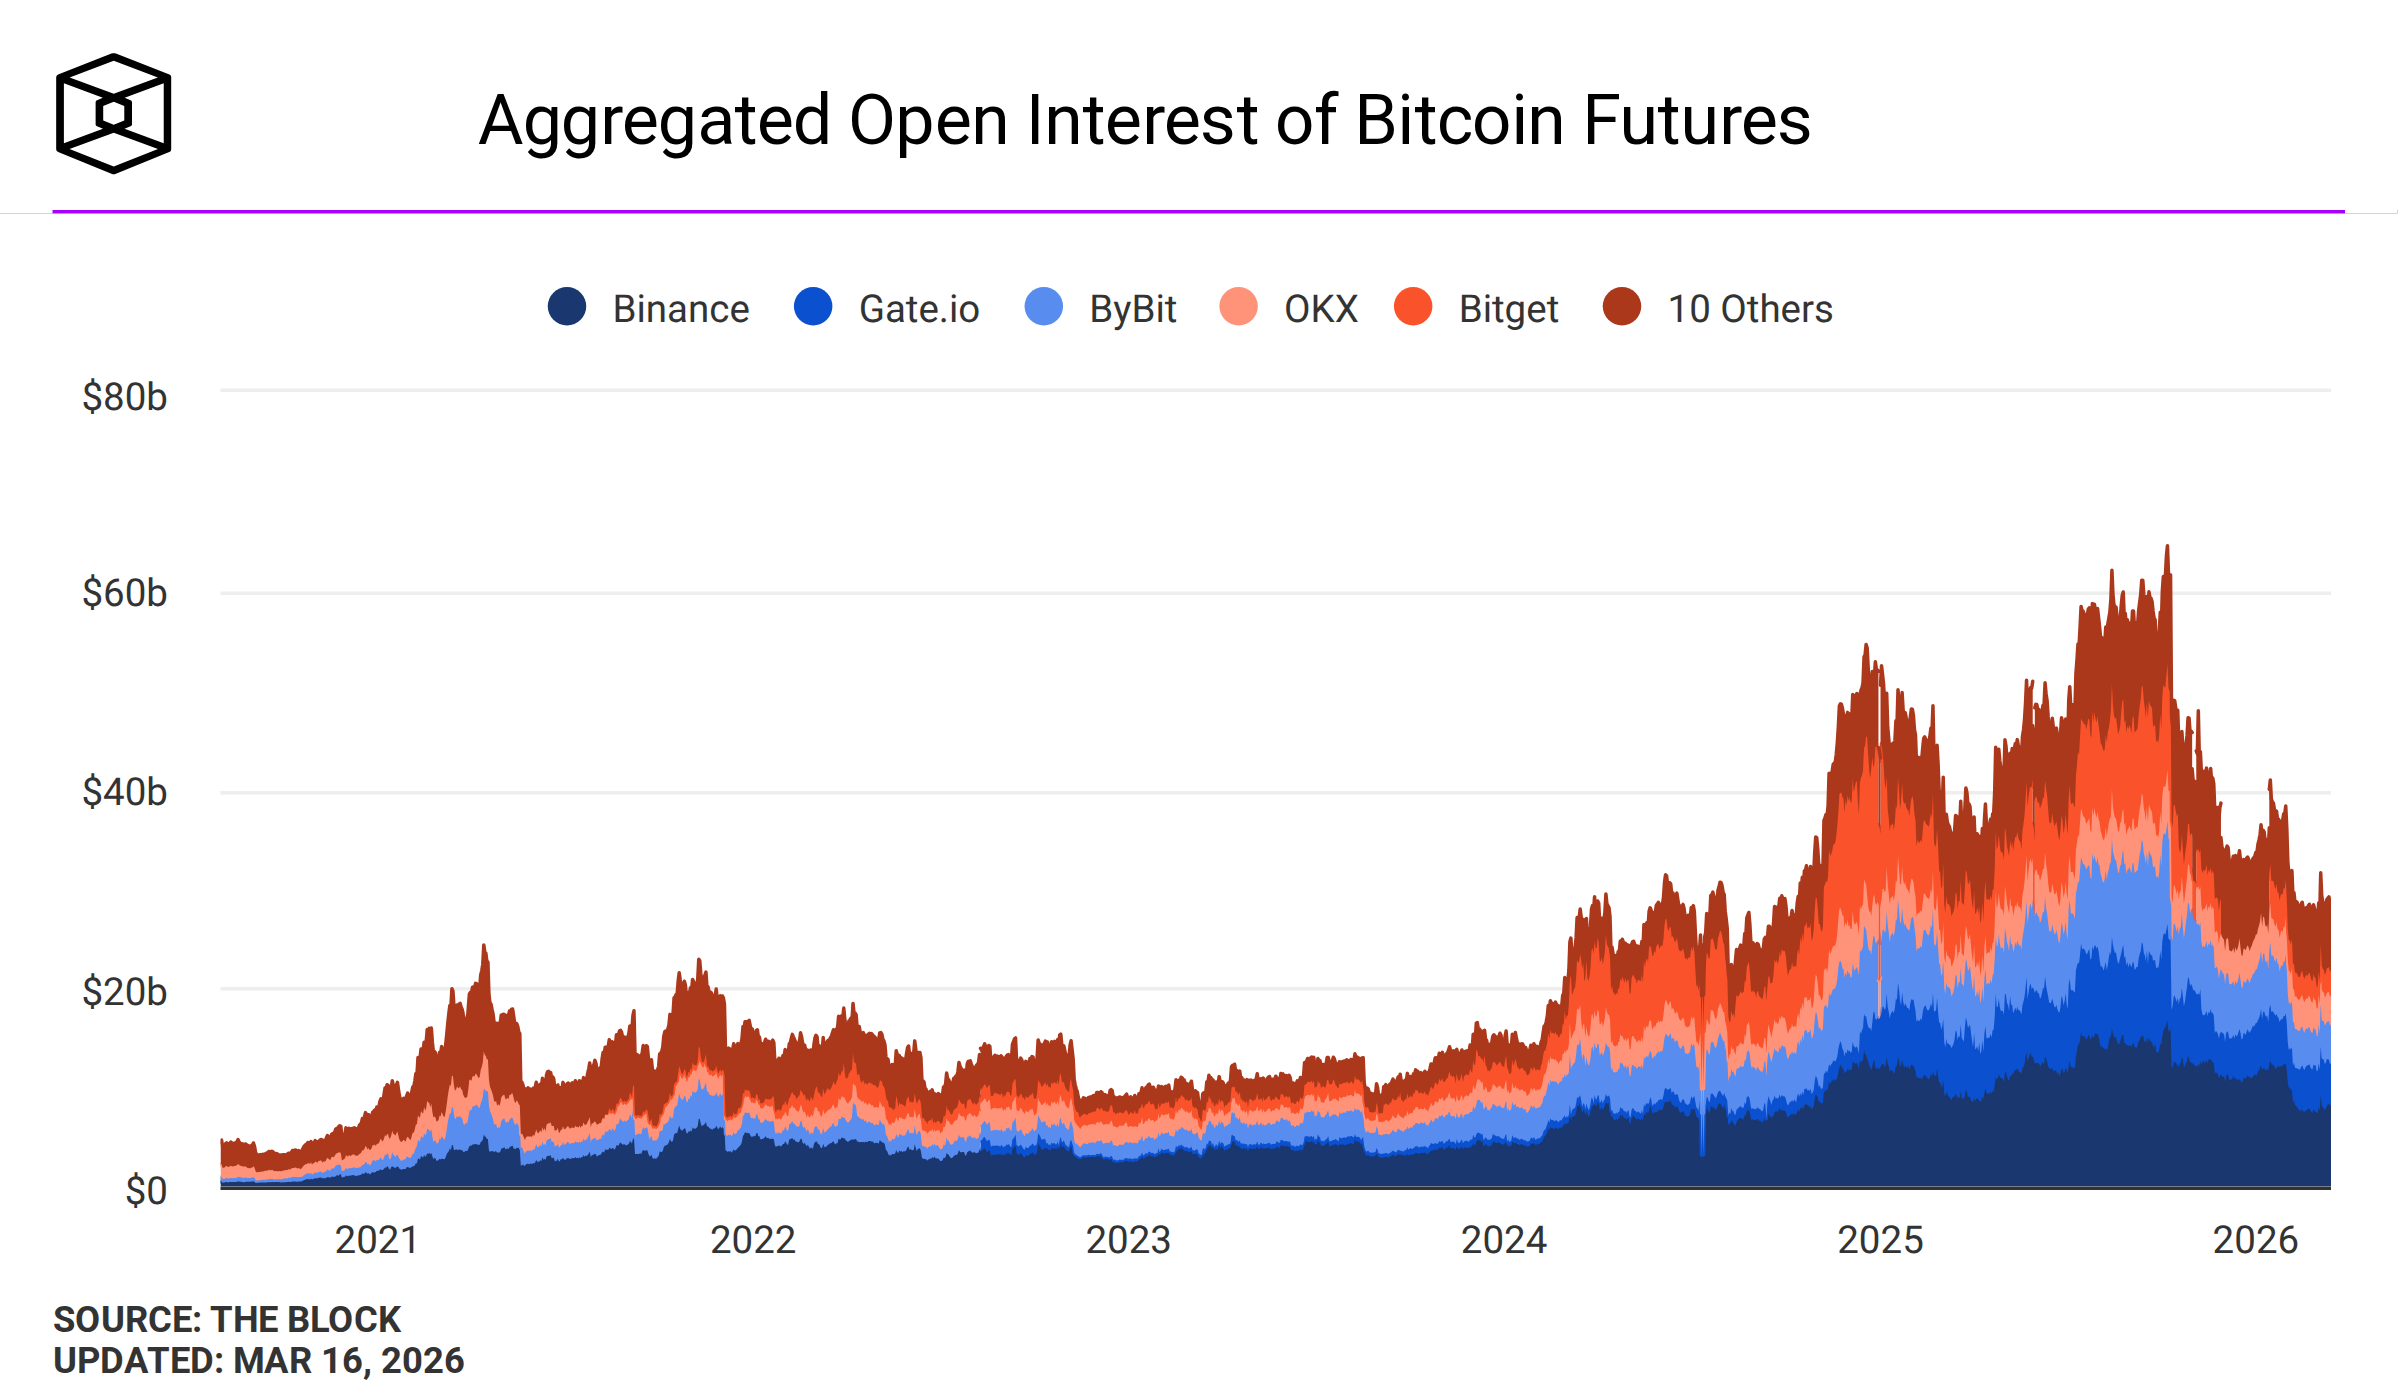
\includegraphics[width=1\linewidth]{Figures/aggregated-open-interest-of-bitcoin-futures-daily.png}
\caption{Bitcoin futures open interest across major exchanges. Source: theblock.co}
    \label{fig:BTC ETF}
\end{figure} 

  % \vspace{0.3em}
  % % FIGURE PLACEHOLDER: Two-panel figure
  % % Left: CME Bitcoin futures volume and open interest (monthly, 2021--2025)
  % % Right: Perpetual futures volume across major crypto exchanges (monthly)
  % % Source: The Block, Coinglass
  % \textit{[Figure: CME futures OI/volume and crypto exchange perpetual futures volume. Source: theblock.co / Coinglass]}
\end{frame}


\begin{frame}{Reading Funding Rates}
  Funding rates on perpetual futures contain information about \highlight{market positioning and sentiment}.
  
  \vspace{0.5em}
  \textbf{Interpretation:}
  \begin{center}
    \small
    \begin{tabular}{lll}
      \toprule
      \textbf{Funding rate} & \textbf{Price trend} & \textbf{Signal} \\
      \midrule
      High positive & Rising & Crowded long---potential correction \\
      Low / negative & Falling & Crowded short---potential reversal \\
      Declining & Rising & Shorts growing despite rally---divergence \\
      Rising & Falling & Longs adding despite decline---divergence \\
      \bottomrule
    \end{tabular}
  \end{center}
  
  \vspace{0.5em}
  \textbf{Economic intuition}: Extreme funding rates indicate one-sided positioning. When most traders are on the same side, small price moves can trigger cascading liquidations, amplifying volatility.
  
  % \vspace{0.3em}
  % % FIGURE PLACEHOLDER: BTC funding rates (7DMA, annualised) across major exchanges
  % % Source: The Block — "BTC Funding Rates (7DMA, APY)"
  % \textit{[Figure: BTC perpetual futures funding rates over time. Source: theblock.co]}
  
  \vspace{0.3em}
  \textbf{Basis trade opportunity}: Some institutional investors buy spot BTC (or the ETF) and short futures to earn the funding rate---a strategy called \textbf{cash-and-carry}. This is a real, measurable return and has attracted significant capital since ETF approval.
\end{frame}


\begin{frame}{Reading Funding Rates}

  \begin{figure}
    \centering
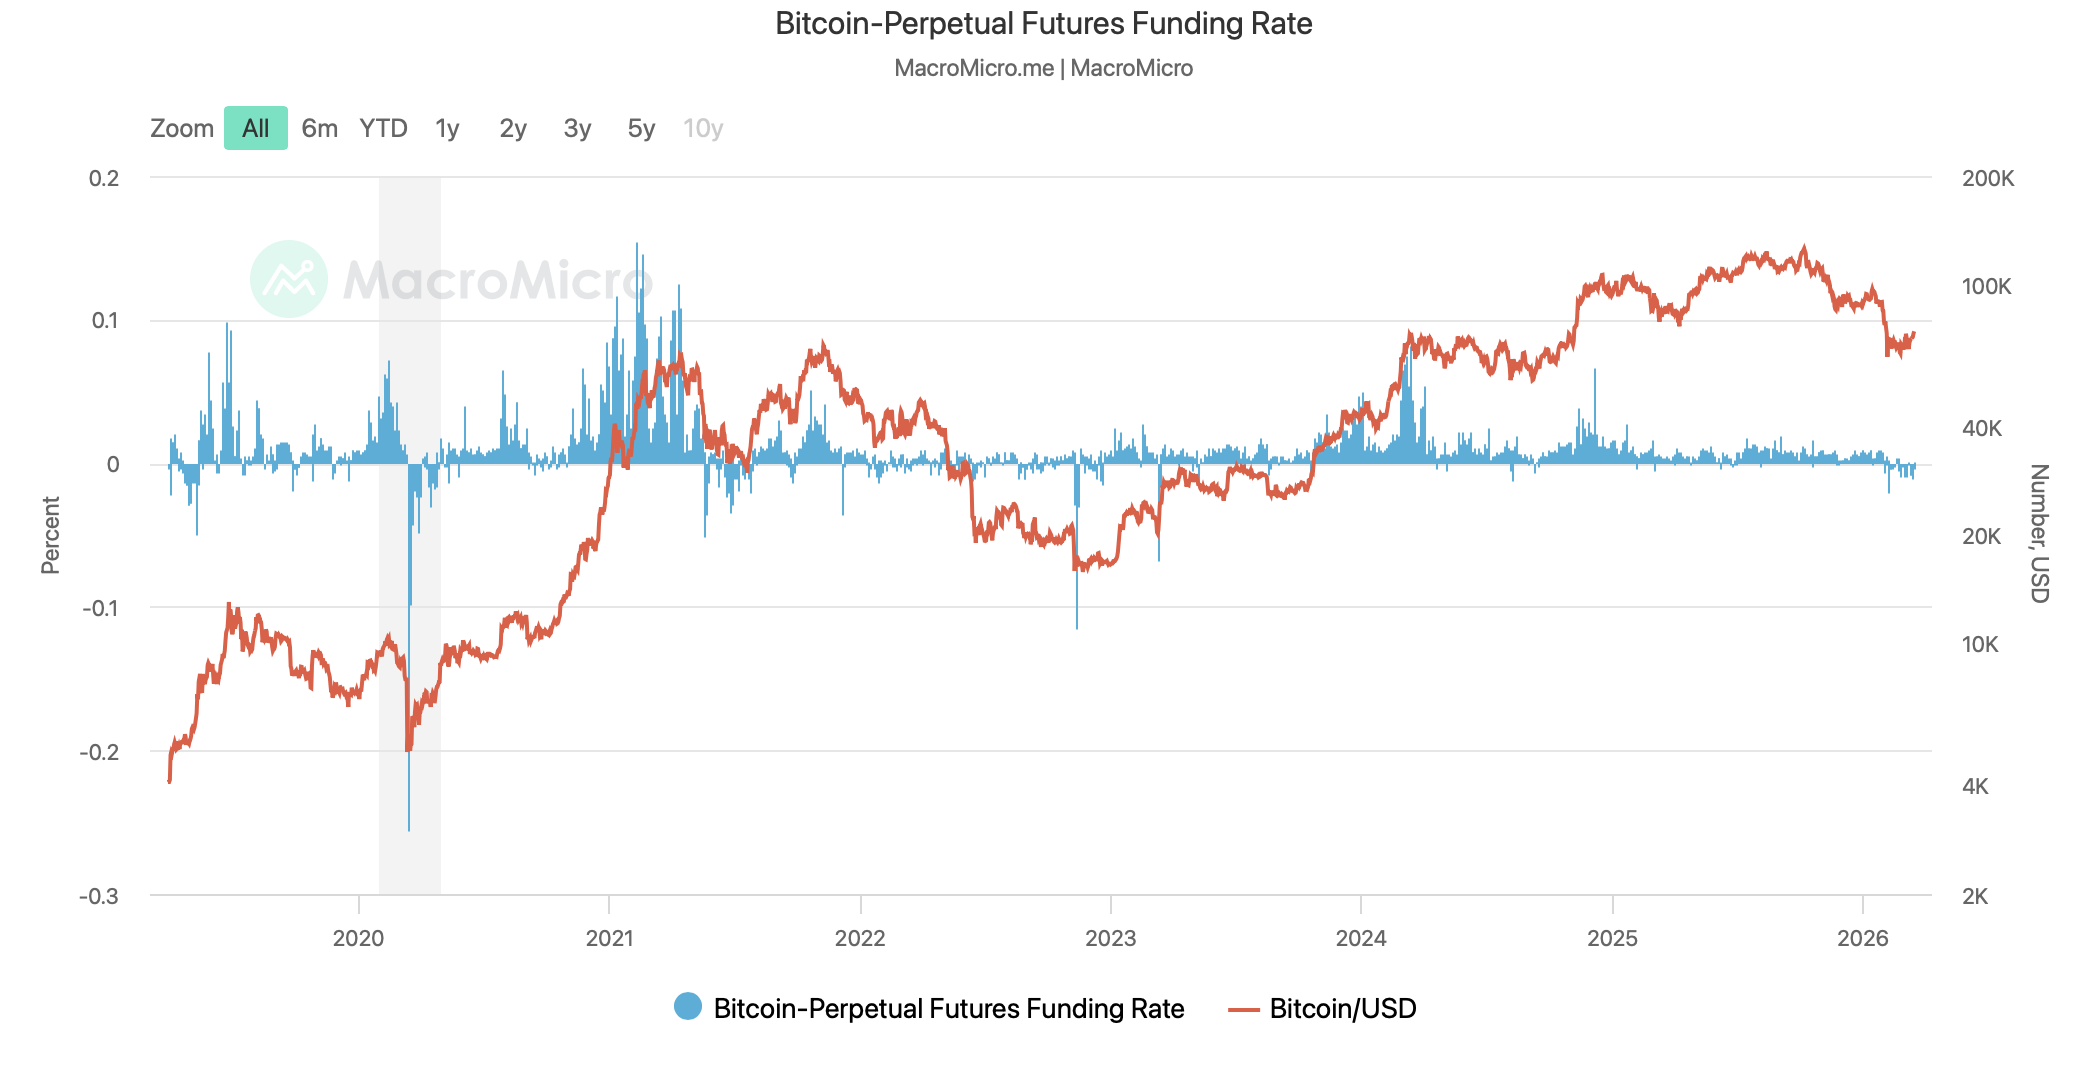
\includegraphics[width=1\linewidth]{Figures/BTC Funding rates.png}
\caption{BTC funding rates (7DMA, annualised) across major exchanges. Source: https://en.macromicro.me}
    \label{fig:BTC Funding Rates}
\end{figure} 

  % \vspace{0.3em}
  % % FIGURE PLACEHOLDER: BTC funding rates (7DMA, annualised) across major exchanges
  % % Source: The Block — "BTC Funding Rates (7DMA, APY)"
  % \textit{[Figure: BTC perpetual futures funding rates over time. Source: theblock.co]}
  
\end{frame}


\begin{frame}{Options Markets}
  Bitcoin options have grown rapidly, primarily on Deribit (dominant, $>$85\% market share) and the CME.
  
  \vspace{0.5em}
  \textbf{Why options matter:}
  \begin{itemize}
    \item \textbf{Hedging}: Protective puts allow holders to limit downside
    \item \textbf{Income generation}: Covered call writing generates yield on BTC holdings
    \item \textbf{Market information}: Option prices reveal the market's expectations about future volatility (implied volatility) and the probability of extreme moves
  \end{itemize}
  
  \vspace{0.5em}
  \textbf{Current state:}
  \begin{itemize}
    \item BTC options open interest: multi-billion dollar notional
    \item Growing institutional use, but still thin compared to equity options
    \item Put/call ratios and implied volatility surfaces are increasingly used by analysts for sentiment and risk assessment
  \end{itemize}
  
  % \vspace{0.3em}
  % % FIGURE PLACEHOLDER: BTC options volume and open interest (CME + Deribit)
  % % Source: The Block — "Volume of Bitcoin Options" and "Volume and OI of CME Bitcoin Options"
  % \textit{[Figure: BTC options volume and open interest. Source: theblock.co]}
\end{frame}


\begin{frame}{Options Markets}

  \begin{figure}
    \centering
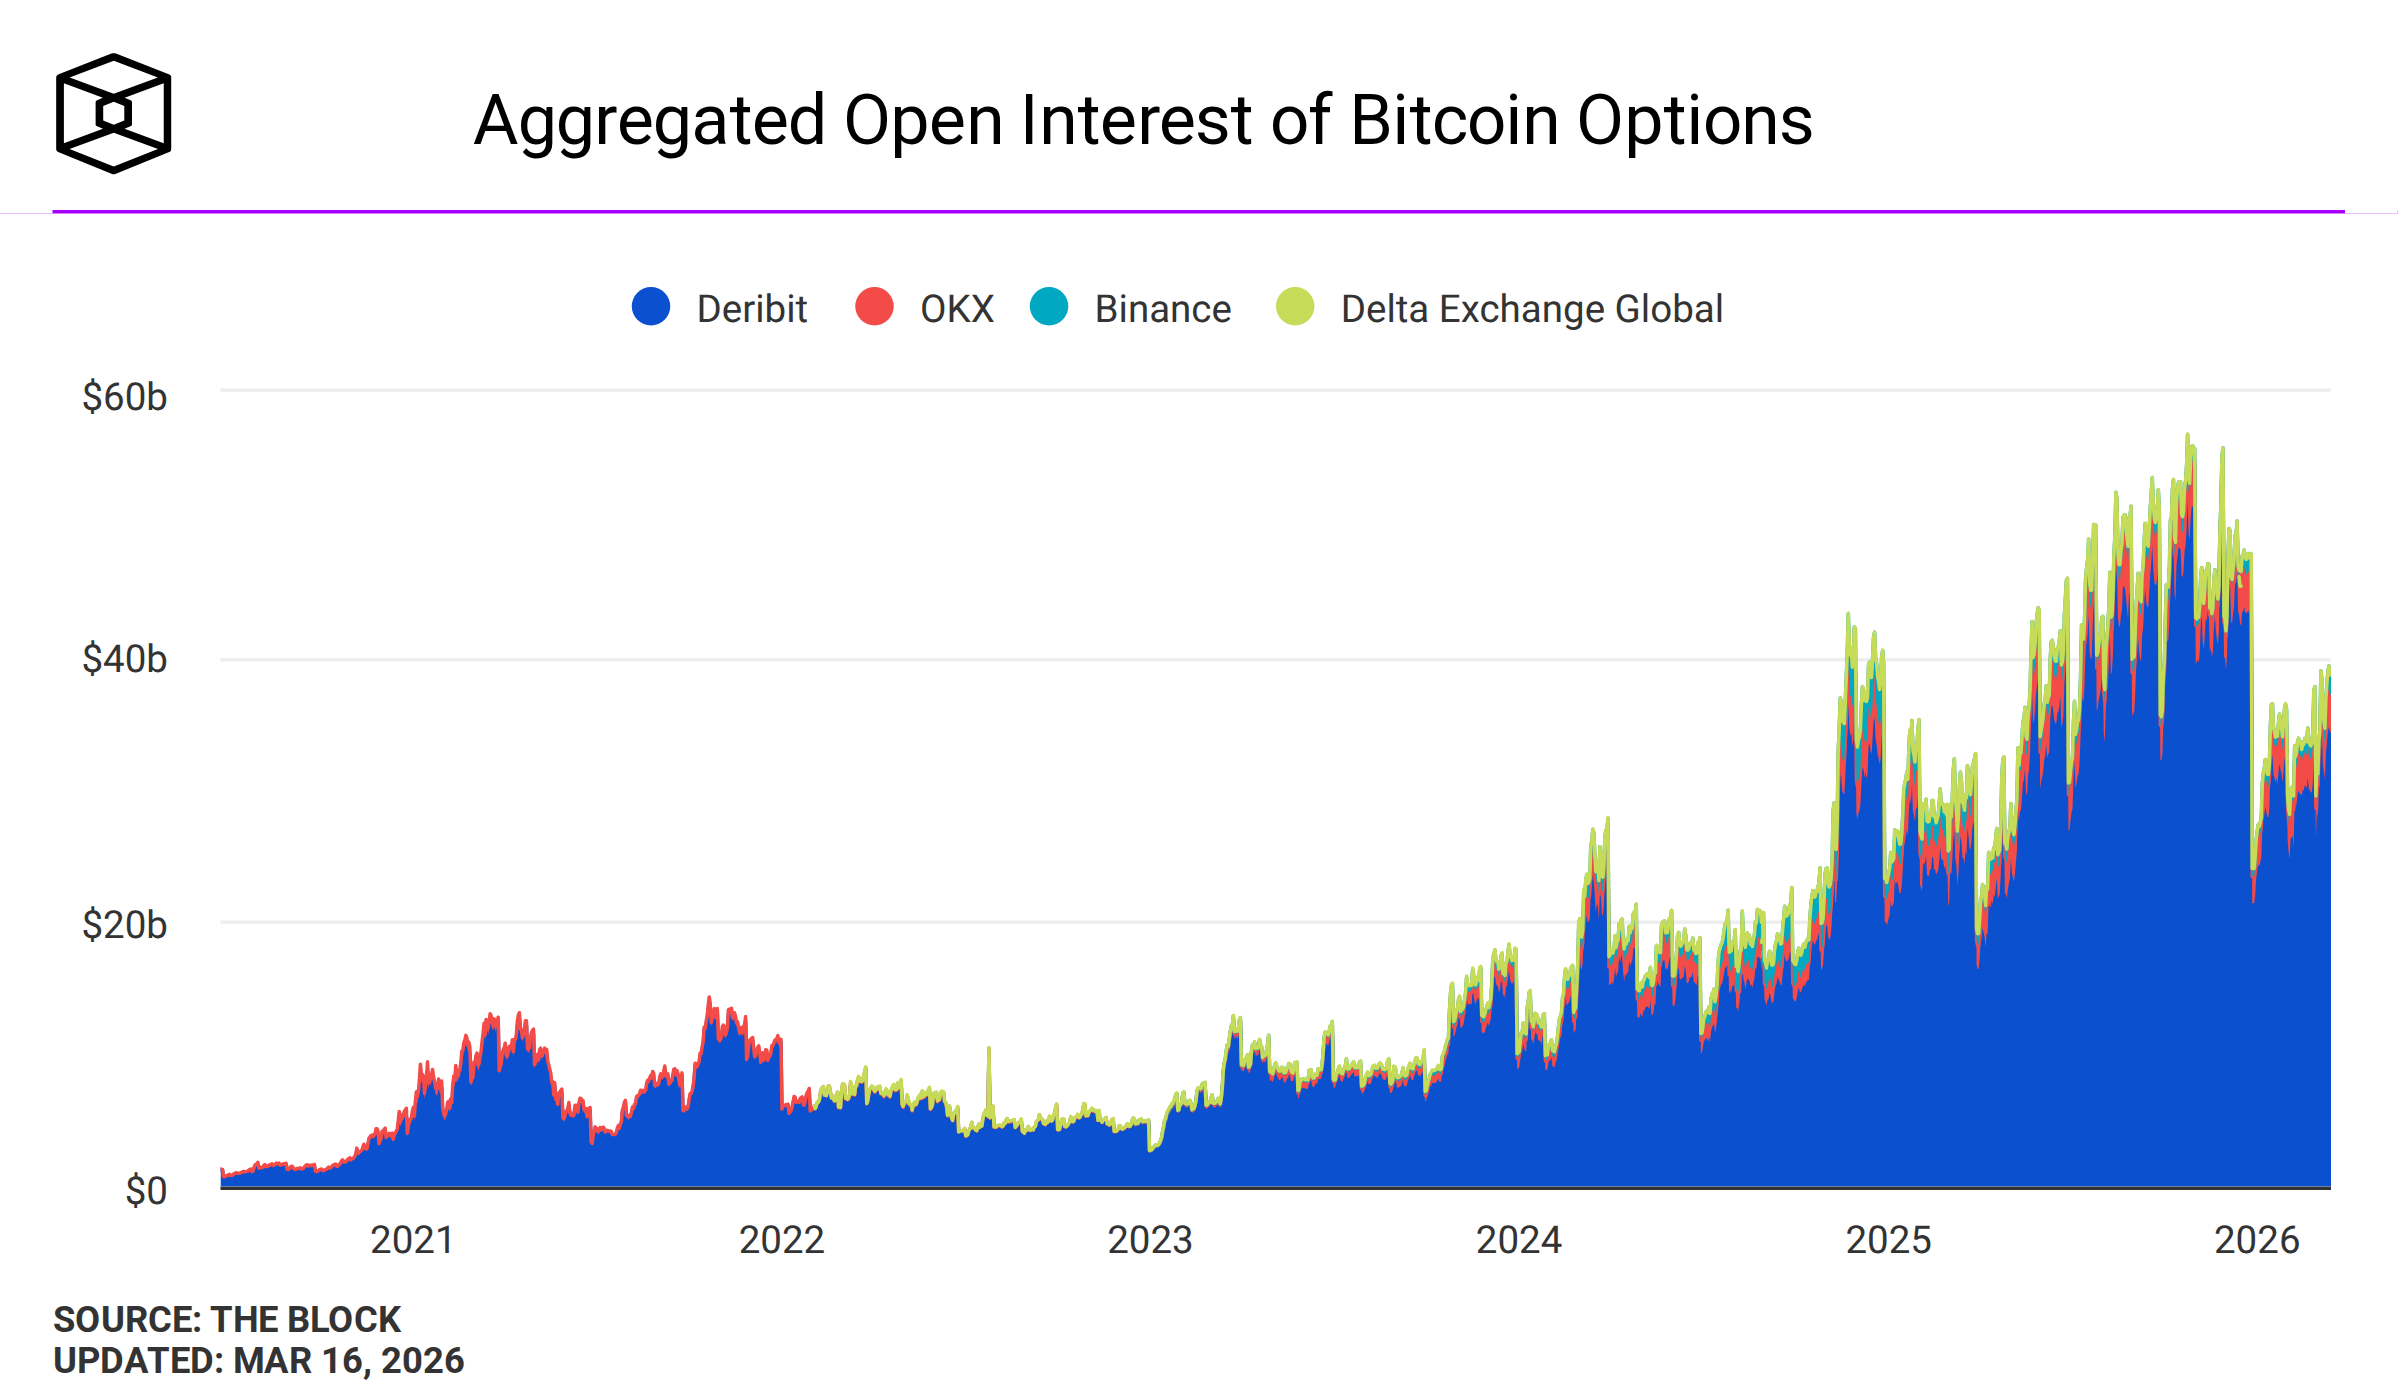
\includegraphics[width=1\linewidth]{Figures/aggregated-open-interest-of-bitcoin-options.png}
\caption{BTC options open interest across exchanges. Source: theblock.co}
    \label{fig:BTC Option Volume}
\end{figure} 
  
  % \vspace{0.3em}
  % % FIGURE PLACEHOLDER: BTC options volume and open interest (CME + Deribit)
  % % Source: The Block — "Volume of Bitcoin Options" and "Volume and OI of CME Bitcoin Options"
  % \textit{[Figure: ]}
\end{frame}

%----------------------------------------------------------------------------------------
\section{Investment Vehicles: A Summary}
%----------------------------------------------------------------------------------------

\begin{frame}{Direct vs.\ Indirect Exposure}
  Investors can access crypto through a range of channels with different risk profiles:
  
  \begin{center}
    \small
    \begin{tabular}{p{3cm}p{3.5cm}p{3.5cm}}
      \toprule
      & \textbf{Direct} & \textbf{Indirect} \\
      \midrule
      \textbf{What you hold} & The token itself & A financial product referencing the token \\
      \textbf{Custody} & Self or third-party & Fund custodian \\
      \textbf{Regulation} & Varies by jurisdiction & Securities regulation \\
      \textbf{Counterparty risk} & Exchange risk & Fund issuer risk \\
      \textbf{Fees} & Trading fees, gas & Management fees \\
      \textbf{Flexibility} & Full (DeFi, staking, etc.) & Limited to product features \\
      \textbf{Tax treatment} & Complex, varies & Standard capital gains \\
      \bottomrule
    \end{tabular}
  \end{center}
  
  \vspace{0.5em}
  The choice between direct and indirect depends on the investor's \textbf{sophistication, regulatory environment, and investment objectives}. Most institutional capital now enters through indirect channels (ETFs, funds, futures).
\end{frame}

\begin{frame}{Direct Investment Channels}
  \textbf{1.\ Buy and hold} (via CEX or DEX):
  \begin{itemize}
    \item Purchase on exchange, withdraw to personal wallet
    \item Full ownership and control; full responsibility for security
  \end{itemize}
  
  \vspace{0.3em}
  \textbf{2.\ Active trading:}
  \begin{itemize}
    \item Higher frequency buying and selling on exchanges
    \item Requires market knowledge; higher transaction costs
    \item Evidence from traditional markets suggests most retail traders \textit{underperform} passive strategies net of costs
  \end{itemize}
  
  \vspace{0.3em}
  \textbf{3.\ DeFi participation} (covered in this course):
  \begin{itemize}
    \item Staking, liquidity provision, lending
    \item Generates yield but introduces impermanent loss and specific risks
    \item This is direct investment \textit{plus} active strategy risk
  \end{itemize}
  
  \vspace{0.3em}
  N.B.\ Direct investment requires managing \textbf{private keys, tax reporting, and regulatory compliance}---barriers that are non-trivial for retail investors and prohibitive for most institutions.
\end{frame}

\begin{frame}{Indirect Investment Channels}
  \textbf{1.\ Spot ETFs} (most significant development):
  \begin{itemize}
    \item Covered in detail earlier this lecture
    \item Regulated, accessible, low fees, no custody burden
    \item Now the dominant institutional on-ramp
  \end{itemize}
  
  \vspace{0.3em}
  \textbf{2.\ Crypto-related equities:}
  \begin{itemize}
    \item Public companies with significant crypto exposure: MicroStrategy, Coinbase (COIN), Marathon Digital (MARA), Riot Platforms (RIOT)
    \item Provides equity-market-regulated exposure with crypto beta
    \item \bad{Company-specific risk} layered on top of crypto risk (management, business model, leverage)
  \end{itemize}
  
  \vspace{0.3em}
  \textbf{3.\ Crypto funds} (hedge funds, venture capital):
  \begin{itemize}
    \item Active management of crypto portfolios
    \item Typically restricted to accredited/institutional investors
    \item Higher fees (2\% management + 20\% performance is common)
    \item Mixed track record (e.g., collapse of Three Arrows Capital, 2022)
  \end{itemize}
\end{frame}

%----------------------------------------------------------------------------------------
\section{Market Integrity and Manipulation}
%----------------------------------------------------------------------------------------

\begin{frame}{Why Market Integrity Matters}
  For crypto to function as a legitimate asset class, markets must be \highlight{fair and orderly}. Without confidence in market integrity, institutional participation is limited and retail investors are at risk.
  
  \vspace{0.5em}
  \textbf{Traditional market safeguards:}
  \begin{itemize}
    \item Securities laws prohibit insider trading and market manipulation
    \item Exchanges conduct real-time surveillance
    \item Self-regulatory organisations (FINRA in the US, FCA in the UK) monitor broker-dealer conduct
    \item Consolidated audit trails enable investigation after the fact
  \end{itemize}
  
  \vspace{0.5em}
  \textbf{Crypto market gaps:}
  \begin{itemize}
    \item Most trading volume occurs on venues outside the reach of regulators
    \item No comprehensive market surveillance across venues
    \item Pseudonymous trading makes identifying manipulators difficult
    \item Insider trading in token listings and protocol upgrades is common and largely unpunished
  \end{itemize}
\end{frame}

\begin{frame}{Types of Manipulation in Crypto Markets}
  \textbf{1.\ Wash trading:}
  \begin{itemize}
    \item Simultaneously buying and selling to inflate volume
    \item Studies estimate 50--70\% of reported exchange volume may be artificial
    \item Motivation: attract listings, earn trading rewards, inflate exchange rankings
  \end{itemize}
  
  \vspace{0.3em}
  \textbf{2.\ Pump and dump:}
  \begin{itemize}
    \item Coordinated buying to inflate a low-cap token's price, followed by selling to latecomers
    \item Often organised via Telegram/Discord groups
    \item Primarily affects small-cap tokens; less relevant for BTC/ETH
  \end{itemize}
  
  \vspace{0.3em}
  \textbf{3.\ Spoofing:}
  \begin{itemize}
    \item Placing large orders with no intention to execute, to create a false impression of supply or demand
    \item Order is cancelled before execution
    \item Illegal in regulated markets; largely unmonitored in crypto
  \end{itemize}
  
  % \vspace{0.3em}
  % \textbf{4.\ Front-running and MEV:}
  % \begin{itemize}
  %   \item On-chain: Validators/searchers reorder transactions to extract value (Maximal Extractable Value)
  %   \item On exchanges: Insider knowledge of large pending orders
  % \end{itemize}
\end{frame}

\begin{frame}{Case Study: The FTX Collapse (November 2022)}
  FTX was the world's third-largest crypto exchange before its collapse.
  
  \vspace{0.5em}
  \textbf{What happened:}
  \begin{itemize}
    \item FTX mixed customer funds with its trading firm, Alameda Research
    \item Alameda used customer deposits to fund speculative trades and venture investments
    \item When a bank-run-like withdrawal wave hit in November 2022, FTX could not honour redemptions
    \item \$8--10 billion in customer funds were missing
    \item Founder Sam Bankman-Fried convicted of fraud (sentenced to 25 years, March 2024)
  \end{itemize}
  
  \vspace{0.5em}
  \textbf{Lessons for the asset class question:}
  \begin{itemize}
    \item \bad{Counterparty risk} on unregulated exchanges is real and catastrophic
    \item ``Proof of reserves'' is insufficient---you need proof of \textit{liabilities} too
    \item The collapse accelerated the push for regulation and strengthened the case for \textit{regulated} access channels like ETFs
  \end{itemize}
\end{frame}

\begin{frame}{Regulatory Responses to Market Integrity}
  The manipulation and fraud problems have prompted regulatory response.
  
  \vspace{0.5em}
  \textbf{EU---Markets in Crypto-Assets Regulation (MiCA):}
  \begin{itemize}
    \item Comprehensive framework effective from December 2024
    \item Requires licensing for crypto-asset service providers (CASPs)
    \item Prohibits market abuse: insider trading, market manipulation, unlawful disclosure
%    \item Reserve and transparency requirements for stablecoins (discussed in Week 5)
  \end{itemize}
  
  \vspace{0.3em}
  \textbf{US---Fragmented approach:}
  \begin{itemize}
    \item SEC: Asserts jurisdiction over tokens that are ``securities'' %(\textbf{Howey test}: Is it an investment of money, in a common enterprise, with expectation of profit, from the efforts of others?)
    \item CFTC: Treats Bitcoin and Ethereum as ``commodities''
   % \item Ongoing legislative efforts to clarify boundaries
    \item Enforcement-led approach: SEC has brought cases against Ripple, Coinbase, Kraken, and others
  \end{itemize}
  
  \vspace{0.3em}
  \textbf{UK---FCA:}
  \begin{itemize}
    \item Crypto marketing rules tightened (since October 2023)
    \item Registration required for crypto firms operating in the UK
    \item No comprehensive licensing regime yet (lagging behind MiCA)
  \end{itemize}
\end{frame}

% \begin{frame}{The Howey Test and ``Is It a Security?''}
%   The classification of tokens as securities has enormous consequences for how they can be issued, traded, and held.
  
%   \vspace{0.5em}
%   \textbf{The Howey test} (from \textit{SEC v.\ Howey}, 1946): A transaction is a security if it involves:
%   \begin{enumerate}
%     \item An \textbf{investment of money}
%     \item In a \textbf{common enterprise}
%     \item With a reasonable \textbf{expectation of profit}
%     \item Derived primarily from the \textbf{efforts of others}
%   \end{enumerate}
  
%   \vspace{0.5em}
%   \textbf{Implications:}
%   \begin{itemize}
%     \item \textbf{Bitcoin}: Generally \textit{not} a security---no issuer, no common enterprise, no management team
%     \item \textbf{Ethereum}: SEC has declined to classify it definitively; approved ETH ETFs suggest commodity treatment
%     \item \textbf{Most ICO tokens}: Likely securities---sold by identifiable teams to fund development, with investors expecting profit from the team's efforts
%     \item \textbf{Consequence}: If a token is a security, it must be registered with the SEC or qualify for an exemption. Most tokens are not registered, creating legal risk.
%   \end{itemize}
  
%   \vspace{0.3em}
%   This regulatory ambiguity is itself a risk factor for investors and a reason why institutional adoption has concentrated on BTC and ETH.
% \end{frame}

%----------------------------------------------------------------------------------------
\section{Summary and Next Steps}
%----------------------------------------------------------------------------------------

\begin{frame}{Key Takeaways}
  \begin{enumerate}
    \item \textbf{Spot ETFs transformed crypto's accessibility}
    \begin{itemize}
      \item The 2024 approvals were the result of a decade-long regulatory battle
      \item Record-breaking inflows; fee competition driving costs down
      \item But ETFs also make Bitcoin behave more like a correlated risk asset
    \end{itemize}
    
    \vspace{0.3em}
    \item \textbf{Institutional infrastructure is now largely in place}
    \begin{itemize}
      \item Qualified custody, regulated derivatives, prime brokerage
      \item Concentration risk (especially Coinbase) remains a concern
    \end{itemize}
    
    \vspace{0.3em}
    \item \textbf{Multiple investment channels exist with different risk profiles}
    \begin{itemize}
      \item Direct: Full control, full responsibility
      \item Indirect (ETFs, equities, funds): Regulated access, limited flexibility
      \item Derivatives: Leverage, hedging, and sentiment information
    \end{itemize}
    
    \vspace{0.3em}
    \item \textbf{Market integrity remains the weakest link}
    \begin{itemize}
      \item Wash trading, manipulation, and fraud persist on unregulated venues
      \item MiCA, SEC enforcement, and ETF surveillance are partial solutions
      \item Regulatory classification (security vs.\ commodity) is still unresolved for most tokens
    \end{itemize}
  \end{enumerate}
\end{frame}

\begin{frame}{Putting It All Together: The Asset Class Verdict}
  After two weeks of analysis, where does the evidence leave us?
  
  \vspace{0.5em}
  \begin{center}
    \small
    \begin{tabular}{lcc}
      \toprule
      \textbf{Criterion} & \textbf{Assessment} & \textbf{Trend} \\
      \midrule
      Return potential & \good{High} & Moderating with maturity \\
      Risk (volatility, drawdowns) & \bad{Very high} & Declining but still extreme \\
      Liquidity (BTC/ETH) & \good{Adequate} & Improving via ETFs \\
      Liquidity (altcoins) & \bad{Poor} & Fragmented \\
      Regulatory framework & Mixed & Improving (MiCA, ETFs) \\
      Correlation / diversification & \bad{Weakening} & Higher with institutionalisation \\
      Market integrity & \bad{Poor} & Slowly improving \\
%      Valuation anchor & \bad{Absent} & Partial for ETH (yield) \\
      \bottomrule
    \end{tabular}
  \end{center}
  
  \vspace{0.5em}
  \textbf{Bottom line}: Bitcoin and Ethereum are increasingly \textit{investable}---the infrastructure, regulation, and products now exist. 
  \vspace{0.5em}
  
  But ``investable'' is not the same as ``attractive''. Whether crypto \textit{deserves} a place in a diversified portfolio depends on the investor's risk tolerance, time horizon, and willingness to accept that many fundamental questions remain unanswered.
\end{frame}

\begin{frame}{What's Next}
  \textbf{Week 9: Blockchain in Traditional Finance}
  \begin{itemize}
    \item Tokenization of securities: bonds, equities, money market funds
    \item Settlement and clearing: from T+1 to near-instant
    \item Institutional blockchain initiatives (JPMorgan Onyx, DTCC)
    \item Central bank experiments: wholesale CBDCs and cross-border payments
    \item Integration challenges: legacy systems, interoperability, and regulation
  \end{itemize}
  
  \vspace{1em}
  \textbf{Preparation:}
  \begin{itemize}
    \item Think about: Why does it still take one business day to settle a stock trade, when Bitcoin settles in 10 minutes? What are the obstacles to faster settlement?
    \item Explore: Look up BlackRock's BUIDL fund (tokenized treasuries) and compare its structure to a traditional money market fund
  \end{itemize}
\end{frame}

\begin{frame}[plain]
  \vfill
  \begin{center}
    {\Large Questions?}
  \end{center}
  \vfill
\end{frame}

\end{document}